\documentclass[9pt,aspectratio=169]{beamer}

% --- Theme ---
\usetheme{Singapore}
\setbeamertemplate{navigation symbols}{}   % no icons
\setbeamertemplate{mini frames}{}          % no dots in headline
\setbeamercovered{transparent}

% --- Grayscale colors ---
\definecolor{PelloGrayDark}{RGB}{60,60,60}
\definecolor{PelloGray}{RGB}{120,120,120}
\definecolor{PelloGrayLight}{RGB}{235,235,235}
\definecolor{PelloGrayUltraLight}{RGB}{248,248,248}

\usecolortheme[named=PelloGrayDark]{structure}

% --- Blocks ---
\setbeamertemplate{blocks}[rounded][shadow=false]
\setbeamercolor{block title}{fg=white,bg=PelloGrayDark}
\setbeamercolor{block body}{fg=black,bg=PelloGrayLight}
\setbeamercolor{block title example}{fg=white,bg=PelloGrayDark}
\setbeamercolor{block body example}{fg=black,bg=PelloGrayLight}
\setbeamercolor{section in head/foot}{fg=PelloGray,bg=PelloGrayLight}
\setbeamercolor{subsection in head/foot}{fg=PelloGray,bg=PelloGrayLight}
\setbeamercolor{frametitle}{fg=black}

% --- Itemize bullets (optional; keep if you like the style) ---
\setbeamertemplate{itemize item}{\raisebox{0.2em}{\scalebox{.6}{$\bullet$}}}
\setbeamertemplate{itemize subitem}{\raisebox{0.2em}{\scalebox{1}{$-$}}}

% --- Footer: frame numbers ---
\makeatletter
\setbeamertemplate{footline}{%
  \hfill\usebeamerfont{footline}\insertframenumber/\inserttotalframenumber\hspace{1em}\vspace{2pt}
}
\makeatother

% --- Minimal packages (add more only when needed) ---
\usepackage[english]{babel}
\usepackage[T1]{fontenc}
\usepackage[utf8]{inputenc}
\usepackage{graphicx}
\usepackage{tikz}
\usepackage{booktabs}
\usepackage{makecell} % for jumping lines within cells in tables.
\usepackage{multirow}
\usepackage{amsmath}
\usepackage{hyperref}
\hypersetup{colorlinks,linkcolor=,urlcolor=blue}
\usepackage{comment}
\usepackage{listings}
\lstset{
  language=R,
  basicstyle=\ttfamily\footnotesize,
  keywordstyle=\color{blue},
  commentstyle=\color{green!50!black},
  stringstyle=\color{red},
  frame=single,
  showstringspaces=false
}
\linespread{1.7}   % 1.0 = normal, 1.2–1.5 common
\AtBeginEnvironment{lstlisting}{\linespread{1}\selectfont} % keep code listings single-spaced

% --- Meta ---
\title{Applied Economics}
\subtitle{Data and Plotting}
\author{Pello Aspuru}
%\institute{University of Vienna}
\date{Winter 2026/2027}

% --- Title page spacing + bottom-left author/date ---
\setbeamertemplate{title page}{
  \vspace{8em}
  \begin{center}
	{\usebeamerfont{title}\inserttitle\par}
  	\vspace{1.5em} % <-- increase title–subtitle gap
  {\usebeamerfont{subtitle}\insertsubtitle\par}
  \end{center}
  \vspace{4em}
  \begin{flushleft}
    {\usebeamerfont{author}\insertauthor\par}
    {\usebeamerfont{date}\insertdate}
  \end{flushleft}
}

\begin{document}

% Title slide without headline/footer
{
  \setbeamertemplate{headline}{}
  \setbeamertemplate{footline}{}
  \begin{frame}
    \titlepage
  \end{frame}
}

\section{Data}

\begin{frame}{Types of Variables in a Dataset}
\linespread{1.2}\selectfont

\begin{center}
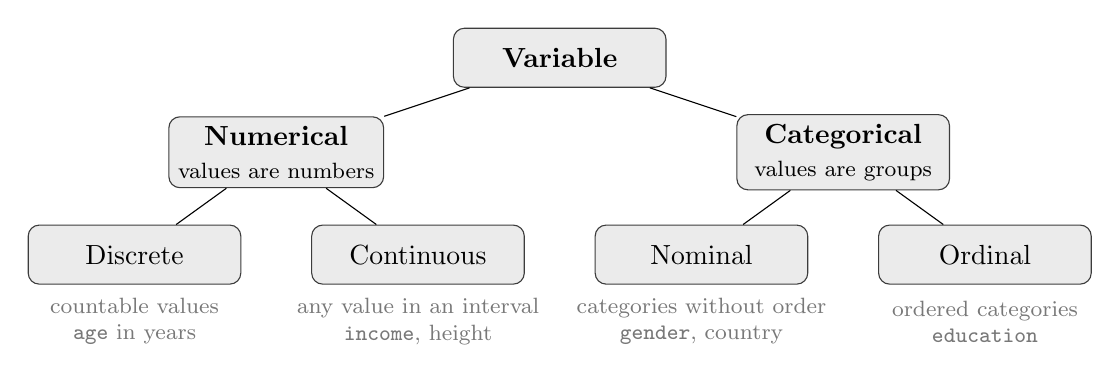
\begin{tikzpicture}[
  box/.style={draw=PelloGrayDark, rounded corners, fill=PelloGrayLight, align=center, minimum width=2.7cm, minimum height=0.75cm},
  ex/.style={align=center, font=\footnotesize, text=PelloGray}]
  \node[box] (var) at (0,0) {\textbf{Variable}};
  \node[box] (num) at (-3.6,-1.2) {\textbf{Numerical}\\ \footnotesize values are numbers};
  \node[box] (cat) at (3.6,-1.2) {\textbf{Categorical}\\ \footnotesize values are groups};
  \node[box] (dis) at (-5.4,-2.5) {Discrete};
  \node[box] (con) at (-1.8,-2.5) {Continuous};
  \node[box] (nom) at (1.8,-2.5) {Nominal};
  \node[box] (ord) at (5.4,-2.5) {Ordinal};
  \node[ex] at (-5.4,-3.35) {countable values\\ \texttt{age} in years};
  \node[ex] at (-1.8,-3.35) {any value in an interval\\ \texttt{income}, height};
  \node[ex] at (1.8,-3.35) {categories without order\\ \texttt{gender}, country};
  \node[ex] at (5.4,-3.35) {ordered categories\\ \texttt{education}};
  \draw (var) -- (num); \draw (var) -- (cat);
  \draw (num) -- (dis); \draw (num) -- (con);
  \draw (cat) -- (nom); \draw (cat) -- (ord);
\end{tikzpicture}
\end{center}

\pause
\begin{itemize}
  \item A \textbf{binary} (dummy) variable is a categorical variable with two categories, coded as 0 and 1: \texttt{employed}.
  \item In R, \texttt{class(df\$income)} returns the type of a variable: \texttt{numeric} or \texttt{integer} for numerical variables, \texttt{character} or \texttt{factor} for categorical ones.
\end{itemize}
\end{frame}

\begin{frame}{Importing and Saving Data}

        \begin{itemize}
    \item \color{teal} .Rdata\color{black} 
    
    \texttt{load("filename.RData"),\\ save(object, file = "filename.RData")}
    \item  \color{teal} .csv \color{black}
    
    \texttt{read.csv("filename.csv"),\\ write.csv(object, file = "filename.csv")}
    \item  \color{teal}.xls \color{black} \texttt{read\_xls("filename.xls")} from package \textit{readxl}
    \item  \color{teal}.dta  \color{black}\texttt{read\_dta("filename.xls")} from package \textit{haven}
\end{itemize}
\end{frame}


\begin{frame}[fragile]{Plotting Data with ggplot2}


\begin{lstlisting}[language=R, basicstyle=\ttfamily\small, frame=single]
  install.packages("ggplot2")
  library(ggplot2)
\end{lstlisting}
\pause
\begin{lstlisting}[language=R, basicstyle=\ttfamily\small, frame=single]
# Histogram of income
  ggplot(df, aes(x = income)) +
  geom_histogram(bins = 30) +
  labs(x = "Income", y = "Frequency")
\end{lstlisting}
\pause 
\begin{lstlisting}[language=R, basicstyle=\ttfamily\small, frame=single]
# Scatterplot of income against age
ggplot(df, aes(x = income, y = age)) +
  geom_point(size  = 2) +
  labs(x = "Income", y = "Age")
\end{lstlisting}

\end{frame}

\section{Graphs}

% Figures: pages of w1_graphs.pdf, built by w1_figures.R from w1_code.R in ../AE_week01_Intro (copy it here after rebuilding)
\newcommand{\graphfig}[1]{\includegraphics[width=0.9\linewidth,page=#1]{w1_graphs.pdf}}

\begin{frame}{Main Types of Graphs in Economic Research}
\linespread{1.3}\selectfont

Which graph to use depends on \textbf{how many} variables you want to show and on their \textbf{type}:

\begin{itemize}
  \item \textbf{Continuous} variables take many numerical values (income, age, GDP).
  \item \textbf{Categorical} variables take a few values or labels (gender, education, country).
\end{itemize}

\medskip
\begin{center}
\small
\begin{tabular}{llll}
\toprule
\textbf{Graph} & \textbf{Variables} & \textbf{Shows} & \textbf{ggplot2} \\
\midrule
Histogram    & 1 continuous                 & distribution of a variable          & \texttt{geom\_histogram()} \\
Bar chart    & 1 categorical                & number of observations per category & \texttt{geom\_bar()} \\
Box plot     & 1 continuous + 1 categorical & distribution within each category   & \texttt{geom\_boxplot()} \\
Scatter plot & 2 continuous                 & relationship between two variables  & \texttt{geom\_point()} \\
Line graph   & 1 continuous + time          & evolution of a variable over time   & \texttt{geom\_line()} \\
\bottomrule
\end{tabular}
\end{center}

\medskip
\pause
All of them allow for \textbf{different categories}: a categorical variable can be added as a \color{teal}colour\color{black}, a \color{teal}fill\color{black}, or a \color{teal}separate panel\color{black}.
\end{frame}


\begin{frame}[fragile]{Histogram}
\linespread{1.3}\selectfont
\textbf{One continuous variable.} Each bar counts the observations in an interval (bin). Categories: one panel per category.

\begin{columns}[t]
\begin{column}{0.5\textwidth}
\centering
\graphfig{3}
\begin{lstlisting}[language=R, basicstyle=\ttfamily\scriptsize]
ggplot(df, aes(x = income)) +
  geom_histogram(bins = 20)
\end{lstlisting}
\end{column}
\begin{column}{0.5\textwidth}
\centering
\graphfig{4}
\begin{lstlisting}[language=R, basicstyle=\ttfamily\scriptsize]
ggplot(df, aes(x = income)) +
  geom_histogram(bins = 20) +
  facet_wrap(~ gender, ncol = 1)
\end{lstlisting}
\end{column}
\end{columns}
\end{frame}


\begin{frame}[fragile]{Bar Chart}
\linespread{1.3}\selectfont
\textbf{One categorical variable.} Each bar counts the observations in a category. Categories: one bar per category.

\begin{columns}[t]
\begin{column}{0.5\textwidth}
\centering
\graphfig{5}
\begin{lstlisting}[language=R, basicstyle=\ttfamily\scriptsize]
ggplot(df, aes(x = education)) +
  geom_bar()
\end{lstlisting}
\end{column}
\begin{column}{0.5\textwidth}
\centering
\graphfig{6}
\begin{lstlisting}[language=R, basicstyle=\ttfamily\scriptsize]
ggplot(df, aes(x = education, fill = gender)) +
  geom_bar(position = "dodge") +
  theme(legend.position = "bottom")
\end{lstlisting}
\end{column}
\end{columns}
\end{frame}


\begin{frame}[fragile]{Box Plot}
\linespread{1.3}\selectfont
\textbf{One continuous and one categorical variable.} Each box shows the median and the quartiles of a category. Categories: split each box by a second categorical variable.

\begin{columns}[t]
\begin{column}{0.5\textwidth}
\centering
\graphfig{7}
\begin{lstlisting}[language=R, basicstyle=\ttfamily\scriptsize]
ggplot(df, aes(x = education, y = income)) +
  geom_boxplot()
\end{lstlisting}
\end{column}
\begin{column}{0.5\textwidth}
\centering
\graphfig{8}
\begin{lstlisting}[language=R, basicstyle=\ttfamily\scriptsize]
ggplot(df, aes(x = education, y = income,
               fill = gender)) +
  geom_boxplot() +
  theme(legend.position = "bottom")
\end{lstlisting}
\end{column}
\end{columns}
\end{frame}


\begin{frame}[fragile]{Scatter Plot}
\linespread{1.3}\selectfont
\textbf{Two continuous variables.} Each point is one observation. Categories: one colour (and one fitted line) per category.

\begin{columns}[t]
\begin{column}{0.5\textwidth}
\centering
\graphfig{9}
\begin{lstlisting}[language=R, basicstyle=\ttfamily\scriptsize]
ggplot(df, aes(x = age, y = income)) +
  geom_point()
\end{lstlisting}
\end{column}
\begin{column}{0.5\textwidth}
\centering
\graphfig{10}
\begin{lstlisting}[language=R, basicstyle=\ttfamily\scriptsize]
ggplot(df, aes(x = age, y = income,
               colour = gender)) +
  geom_point() +
  geom_smooth(method = "lm", se = FALSE)
\end{lstlisting}
\end{column}
\end{columns}
\end{frame}


\begin{frame}[fragile]{Line Graph}
\linespread{1.3}\selectfont
\textbf{One continuous variable over time.} Points are connected in time order. Categories: one line per category.

\begin{columns}[t]
\begin{column}{0.5\textwidth}
\centering
\graphfig{11}
\begin{lstlisting}[language=R, basicstyle=\ttfamily\scriptsize]
ggplot(df_ts[df_ts$country == "A", ],
       aes(x = year, y = unemp)) +
  geom_line()
\end{lstlisting}
\end{column}
\begin{column}{0.5\textwidth}
\centering
\graphfig{12}
\begin{lstlisting}[language=R, basicstyle=\ttfamily\scriptsize]
ggplot(df_ts, aes(x = year, y = unemp,
                  colour = country)) +
  geom_line()
\end{lstlisting}
\end{column}
\end{columns}
\end{frame}


\begin{frame}{Graphs: Summary}

\begin{center}
\small
\begin{tabular}{llll}
\toprule
\textbf{Graph} & \textbf{Variables plotted} & \textbf{Adding categories} & \textbf{Variables with categories} \\
\midrule
Histogram    & 1 & panels (\texttt{facet\_wrap}) or \texttt{fill} & 2 \\
Bar chart    & 1 & \texttt{fill}                                  & 2 \\
Box plot     & 2 & \texttt{fill}                                  & 3 \\
Scatter plot & 2 & \texttt{colour} or \texttt{shape}              & 3 \\
Line graph   & 2 & \texttt{colour} or \texttt{linetype}           & 3 \\
\bottomrule
\end{tabular}
\end{center}

\pause
\begin{itemize}
  \item Panels (\texttt{facet\_wrap}) work with every graph, and can be combined with colours to add yet another variable.
  \item Always label the axes and state the units: \texttt{labs(x = "...", y = "...")}.
  \item Later in the course: graphs of \textbf{estimates} rather than raw data (fitted regression lines, coefficients with confidence intervals).
\end{itemize}
\end{frame}


\end{document}

